\documentclass[problem]{mcs}

\begin{pcomments}
  \pcomment{FP_jections_nofunc}
  \pcomment{CH, S14}
  \pcomment{mashup of smaller problems}
  \pcomment{summary of properties part restored by ARM 2/23/17}
\end{pcomments}

\pkeywords{
  composition
  surjection
  injection
  bijection
  total
  function
  infinite
}

%%%%%%%%%%%%%%%%%%%%%%%%%%%%%%%%%%%%%%%%%%%%%%%%%%%%%%%%%%%%%%%%%%%%%
% Problem starts here
%%%%%%%%%%%%%%%%%%%%%%%%%%%%%%%%%%%%%%%%%%%%%%%%%%%%%%%%%%%%%%%%%%%%%

\begin{problem}
Let $R: A \to B$ and $S: B \to C$ be binary relations such that $S
\compose R$ is a bijection and $\card{A} = 2$.

Give an example of such $R,S$ where neither $R$ nor $S$ is a function.
Indicate exactly which properties---total, surjection, function, and
injection---your examples of $R$ and $S$ have.

\hint Let $\card{B}=4$.

\begin{solution}

\begin{figure}

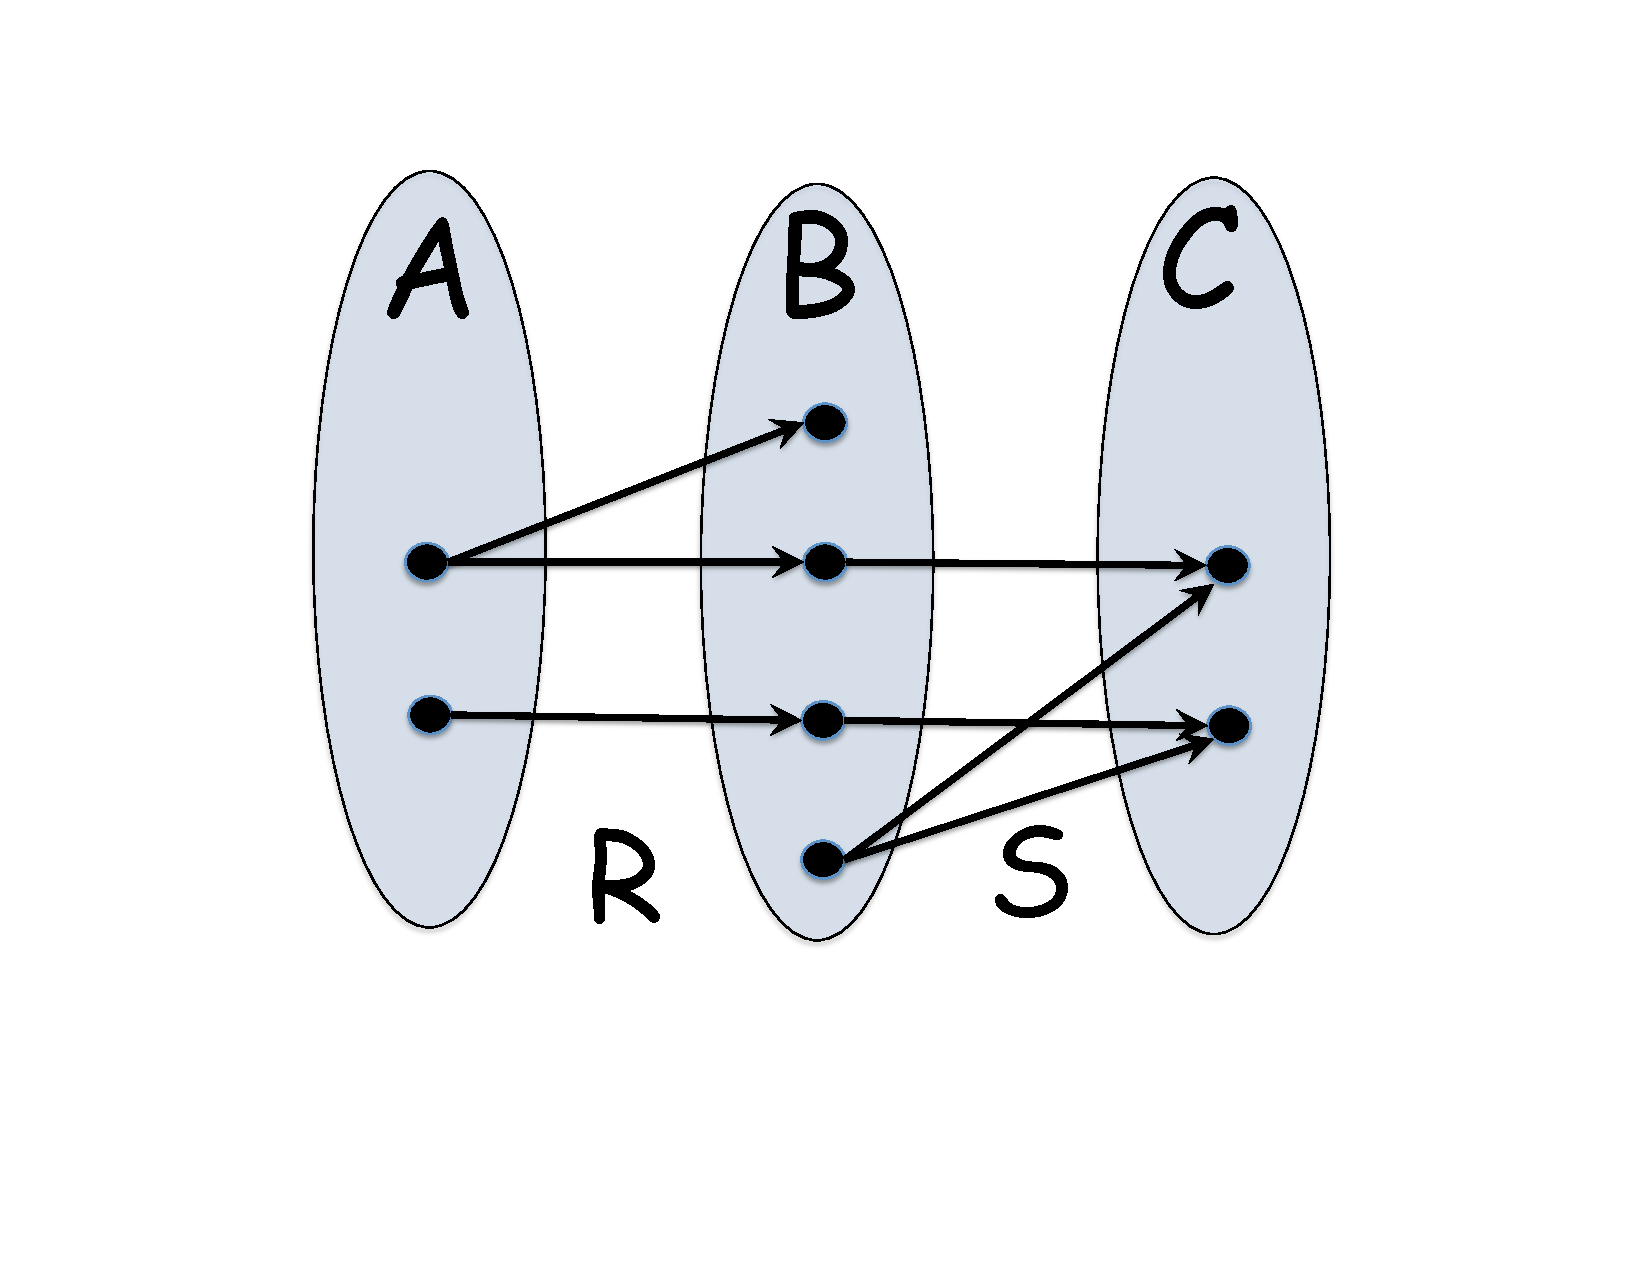
\includegraphics[width = 3.5in]{ScomposeR}

\caption{$S \compose R: A \to C$ is a bijection.}

\label{fig:SoRbij}

\end{figure}

\begin{figure}

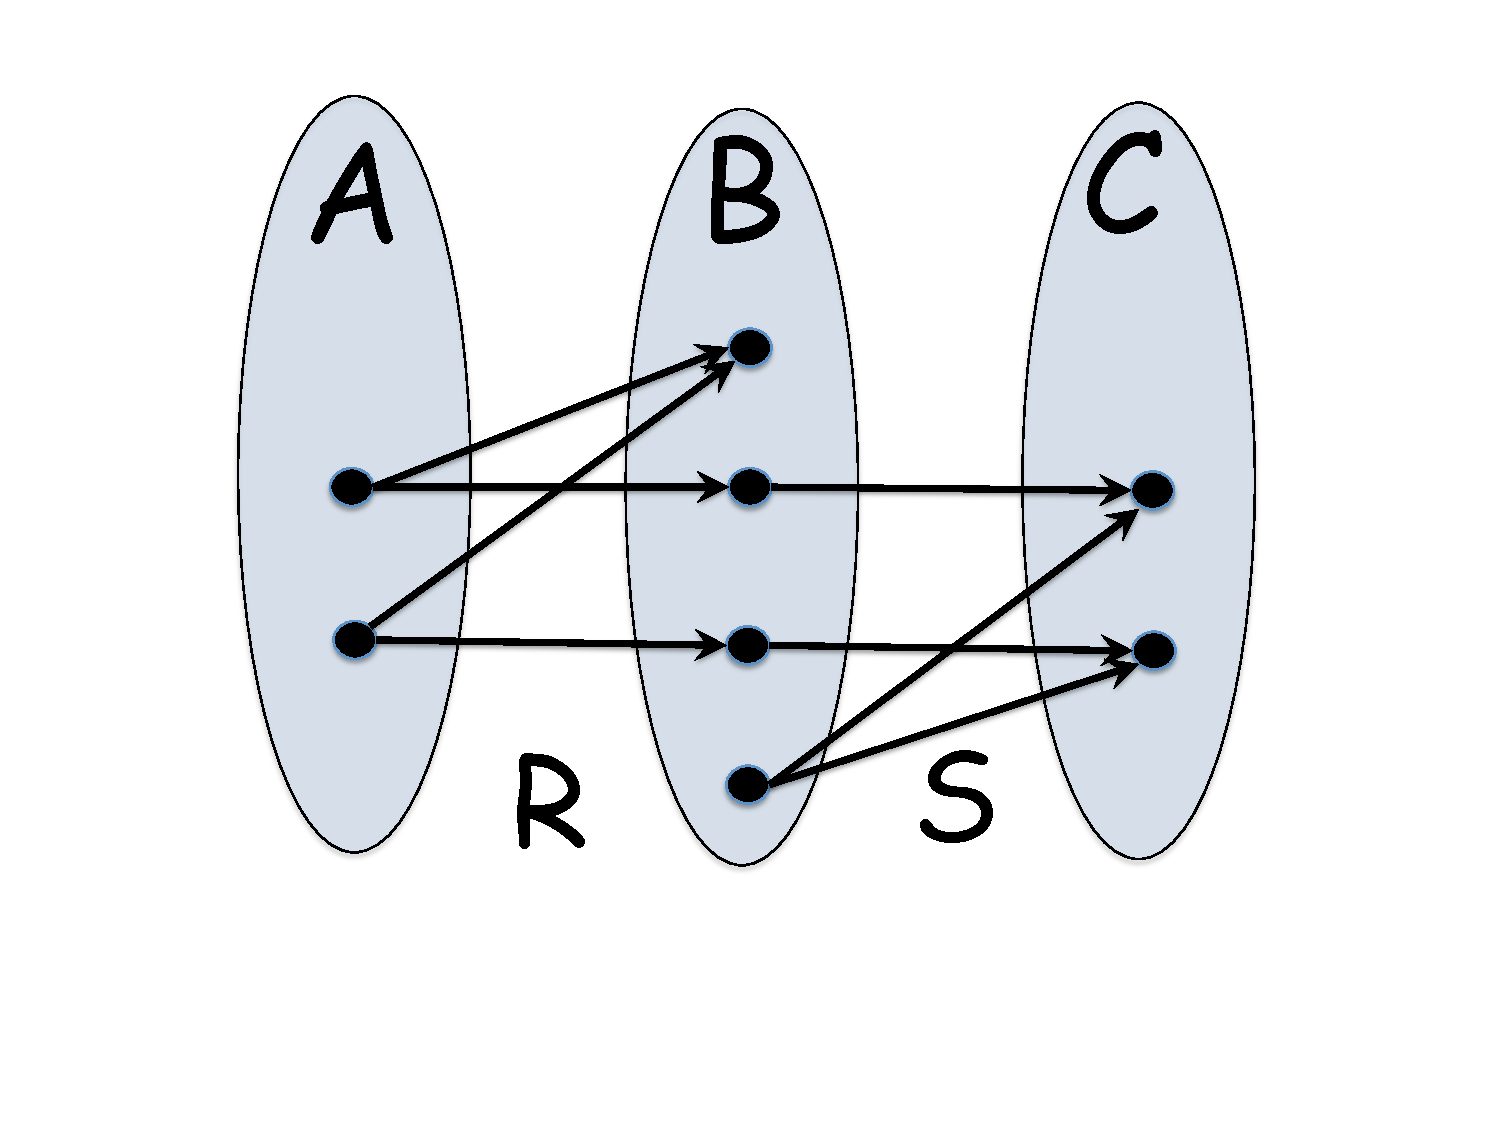
\includegraphics[width = 3.5in]{ScomposeRnoinj}

\caption{$S \compose R: A \to C$ is a bijection and $R$ is not an
  injection.}

\label{fig:SoRbijnoinj}

\end{figure}

It is easy to see that $R$ must be total ($[\geq 1\ \text{out}]$) and
$S$ must be a surjection ($[\ge 1\ \text{in}]$).

$C$ must have 2 elements since $A \bij C$.

For minimal example with $R, S$ not functions, see Figure~\ref{fig:SoRbij}.
For an example in which $R$ is not even an injection, see Figure~\ref{fig:SoRbijnoinj}.

To explain: following the hint, we let $\card{B} = 4$.

We put an $R$-arrow from the first element of $A$ to the second element of
$B$ and an $S$-arrow from this second element of $B$ to the first
element of $C$; likewise from the second element of $A$ to the third
element of $B$ and from this third element of $B$ to the second
element of $C$.  These arrows will provide the bijection defined by $S
\compose R$.

We put two $R$-arrows into the first element in $B$ with no $S$-arrow
out as in Figure~\ref{fig:SoRbijnoinj}; so $R$ is not a function or an
injection and $S$ is not total.  We put two $S$-arrows out of the
fourth element of $B$ and no $R$-arrows in; so $R$ is not a surjection
and $S$ is not a function or an injection.

So besides $R$ being total and $S$ a surjection,
Figure~\ref{fig:SoRbijnoinj} shows that neither $R$ nor $S$ need have
any additional ``jection'' properties. \iffalse That is,
\begin{itemize}

\item $R$ is not a function ($[\leq 1\ \text{out}]$), surjection,
  or injection ($[\leq 1\ \text{in}]$), and

\item $S$ need not be a function, total, or injection.

\end{itemize}
\fi

\end{solution}

\end{problem}

%%%%%%%%%%%%%%%%%%%%%%%%%%%%%%%%%%%%%%%%%%%%%%%%%%%%%%%%%%%%%%%%%%%%%
% Problem ends here
%%%%%%%%%%%%%%%%%%%%%%%%%%%%%%%%%%%%%%%%%%%%%%%%%%%%%%%%%%%%%%%%%%%%%

\endinput

